\documentclass[11pt,a4paper]{article}

% correr en lualatex
\usepackage{fontspec}
\usepackage[spanish,es-tabla]{babel}
\usepackage{csquotes}
\usepackage{geometry}
\geometry{margin=2.5cm}
\usepackage{booktabs}
\usepackage{graphicx}
\usepackage{amsmath}
\usepackage{caption}
\usepackage{subcaption}
\usepackage{threeparttable}
\usepackage{array}
\usepackage[backend=biber,style=authoryear,maxcitenames=2,maxbibnames=99]{biblatex}
\addbibresource{referencias.bib}
\usepackage[colorlinks=true,linkcolor=blue,citecolor=blue,urlcolor=blue]{hyperref}

\captionsetup{font=small,labelfont=bf}
\setlength{\parskip}{0.35em}
\setlength{\parindent}{0pt}
\setlength{\emergencystretch}{3em}

\title{\textbf{Transmisión fiscal y fuga hacia importaciones en Timor-Leste}}
\author{Emerson López \and Julito} %\thanks{} }
\date{\today}

\begin{document}
\maketitle

\begin{abstract}
\noindent
Este documento presenta los resultados del proyecto que estudia cómo responde el PIB real no petrolero de Timor-Leste al gasto público y qué parte del estímulo fiscal se refleja en mayores importaciones. El ejercicio empírico es un VAR bayesiano (BVAR) trimestral con cinco variables endógenas en logaritmos, dos rezagos, dummies de eventos y una identificación recursiva de Cholesky evaluada bajo dos órdenes alternativos. La muestra abarca 2002Q1--2023Q4 (88 trimestres; 86 observaciones efectivas con dos rezagos). Los resultados provienen de los archivos exportados por el proyecto y se describen como evidencia condicionada al modelo y a una muestra corta, no como identificación causal incontrovertible. El shock fiscal se asocia a respuestas positivas y persistentes pero transitorias del gasto, a respuestas positivas del PIB no petrolero con rezago, y a respuestas de las importaciones mayores y más tempranas; la respuesta del índice de precios es positiva pero pequeña, y la del crédito privado no es distinguible de cero con los intervalos posteriores considerados. En el texto, las respuestas se expresan como elasticidades: variaciones porcentuales ante un aumento de 1\% del gasto público.
\end{abstract}

\section{Metodología}
\label{sec:metodologia}

\subsection{Diseño empírico y pregunta}
\label{sec:diseno}

La pregunta central del proyecto es cómo responde el PIB real no petrolero al
gasto público y qué porción del estímulo fiscal se asocia a
mayores importaciones. Timor-Leste es una economía pequeña y abierta, con
una historia macroeconómica corta y series principalmente anuales. Un VAR
bayesiano trimestral permite estimar respuestas dinámicas conjuntas del gasto
público, el PIB no petrolero, las importaciones, los precios y el crédito,
aprovechando la estructura de rezagos y la información previa para contener la
varianza en muestras pequeñas \parencite{litterman1986,giannone2015}.

El diseño sigue la tradición de los VAR estructurales de
\textcite{sims1980}, pero su lectura debe ser prudente: se trata de evidencia
condicionada al modelo, a la desagregación temporal, al prior y al orden
recursivo de identificación, no de identificación causal
incontrovertible. Las importaciones funcionan como canal de fuga externa; el IPC
y el crédito privado permiten observar canales de precios y financieros,
respectivamente.

El objetivo de investigación es estimar cómo responden, a lo largo del tiempo,
el PIB real no petrolero y las importaciones ante un aumento de 1\% del gasto
público, y examinar si esas elasticidades cambian bajo dos órdenes recursivos.
El IPC, el crédito privado y la persistencia del propio gasto son resultados
complementarios. El modelo está en logaritmos y las respuestas se expresan como
elasticidades.

\subsection{Datos, variables y muestra}
\label{sec:datos}

Las cinco variables endógenas, en logaritmos naturales, son:

\begin{table}[htbp]
\centering
\small
\caption{Variables del modelo, unidades y fuentes}
\label{tab:variables}
\resizebox{\textwidth}{!}{%
\begin{tabular}{@{}llll@{}}
\toprule
Variable & Interpretación & Unidades & Fuente principal \\
\midrule
\texttt{ln\_gov\_exp}   & Gasto de consumo final del gobierno & Millones de USD & ADB \parencite{adb2025} \\
\texttt{ln\_gdp\_non}   & PIB real no petrolero               & Millones de USD & ADB \parencite{adb2025} \\
\texttt{ln\_imports}    & Importaciones reales de bienes y servicios & Millones de USD & ADB \parencite{adb2025} \\
\texttt{ln\_cpi}        & Índice de precios al consumidor & Índice & DNE \parencite{dne_cpi} \\
\texttt{ln\_credit}     & Créditos al sector privado      & Millones de USD & ADB \parencite{adb2025} \\
\bottomrule
\end{tabular}}
\par\vspace{0.4em}
\begin{minipage}{0.95\textwidth}
\footnotesize\textit{Nota:} El gasto, el PIB, las importaciones y el crédito se reportan en millones de dólares estadounidenses según las series fuente; el IPC es un índice.
\end{minipage}
\end{table}

La base anual limpia cubre 2002--2023 (22 observaciones). La base trimestral construida cubre 2002Q1--2023Q4 (88 trimestres). Con dos rezagos, el VAR utiliza 86 observaciones efectivas. La muestra es corta
para un VAR de cinco variables y dos rezagos; ello limita la precisión y es
una razón adicional para interpretar los resultados con cautela.

\subsection{Limpieza y construcción de series}
\label{sec:limpieza}

El script \texttt{scripts/01\_cleaning.R} extrae del libro de indicadores del ADB
las cinco series anuales (gasto de consumo final del gobierno, PIB por origen
industrial a precios constantes de 2015, importaciones de bienes y servicios, IPC
de Dili y créditos al sector privado), elimina valores faltantes codificados
y columnas sin información y produce \texttt{timor\_annual\_macro.csv}.

Las importaciones trimestrales de \emph{Trade Map} \parencite{trademap2025} se procesan en el mismo
script: se convierten de miles de USD a millones de USD y se detecta una
observación inusualmente alta en 2010Q4. El script aplica una
corrección registrada en el código: divide ese valor por diez
(\texttt{imports\$imports[36] <- imports\$imports[36] / 10}). Esta decisión
se documenta aquí de forma transparente como el tratamiento aplicado por el
script; no debe presentarse como una corrección inocua ni como un dato
oficial verificado de forma independiente. La serie resultante se guarda en
\texttt{imports\_cleaning\_timor\_leste.csv}. Esa serie se conserva como
insumo de limpieza y comparación, pero no se usa como indicador trimestral en
la desagregación (véase el~\ref{sec:anexo_trademap}).

El IPC mensual se obtiene de la fuente incluida en
\texttt{Data/data-source/CPI Publish Readj New Weight.xls}, que en el propio
archivo se identifica como proveniente de la Direcção Nacional de
Estatística de Timor-Leste \parencite{dne_cpi}. Las observaciones mensuales
disponibles desde 2013 se agregan a frecuencia trimestral mediante promedios
aritméticos y se almacenan en \texttt{cpi\_months.csv}.

\subsection{Desagregación temporal}
\label{sec:desagregacion}

Para evitar tratar observaciones anuales como si fueran de alta frecuencia, las
series anuales se desagregan con el método proporcional de Denton--Cholette
univariado sin indicador trimestral
\parencite{denton1971,cholette1984,tempdisagg}. Para las variables de flujo (gasto
público, PIB real no petrolero e importaciones reales) se impone la
restricción de suma anual:
\[
\sum_{q=1}^{4} x_{t,q} = X_t .
\]
Para el IPC y el crédito privado se impone la restricción de promedio
trimestral. El IPC trimestral desagregado se sustituye desde 2013 por el promedio
trimestral calculado con las observaciones mensuales oficiales. De este modo se
distingue entre observaciones oficiales y estimaciones trimestrales
interpoladas: las primeras son datos observados agregados, mientras que las
segundas son interpolaciones que respetan las restricciones anuales.

El proyecto probó las importaciones de \emph{Trade Map} como indicador
trimestral en una especificación de Chow--Lin. El coeficiente del indicador fue
0.1706 (EE 0.2959; $t=0.576$; $p=0.571$), no significativo, y el $R^2$ ajustado
fue $-0.0328$; la estimación se documenta en el~\ref{sec:anexo_trademap}.
Por eso se descartó esa serie de alta frecuencia y todas las series se
desagregan con el método univariado proporcional de la misma variable anual,
que preserva estrictamente las restricciones anuales oficiales. La
desagregación induce suavidad determinista y autocorrelación en las
series trimestrales; este punto se retoma como limitación en la
sección~\ref{sec:diag}.

\subsection{Quiebres y controles exógenos}
\label{sec:quiebres}

El script \texttt{scripts/03\_structural\_failures.R} estima quiebres
estructurales múltiples con el procedimiento de Bai--Perron y selecciona el
número de quiebres por el criterio BIC \parencite{baiperron1998,baiperron2003}.
La tabla~\ref{tab:quiebres} reproduce las fechas óptimas obtenidas al
reejecutar el análisis sobre los datos del repositorio.

\begin{table}[htbp]
\centering
\small
\begin{threeparttable}
\caption{Quiebres estructurales óptimos por serie (Bai--Perron, selección por BIC)}
\label{tab:quiebres}
\begin{tabular}{@{}lcl@{}}
\toprule
Serie & Número de quiebres & Fechas óptimas (trimestres) \\
\midrule
\texttt{ln\_gov\_exp} & 4 & 2005Q4, 2009Q2, 2012Q4, 2016Q3 \\
\texttt{ln\_gdp\_non} & 4 & 2006Q1, 2010Q3, 2016Q3, 2019Q4 \\
\texttt{ln\_imports}  & 4 & 2005Q4, 2009Q1, 2012Q3, 2020Q3 \\
\texttt{ln\_cpi}      & 4 & 2005Q2, 2009Q1, 2012Q4, 2020Q3 \\
\texttt{ln\_credit}   & 3 & 2005Q1, 2011Q1, 2020Q3 \\
\bottomrule
\end{tabular}
\begin{tablenotes}\footnotesize
\item Nota: Fuente: elaboración propia con \texttt{scripts/03\_structural\_failures.R}. Las fechas se agrupan en ventanas históricas y se resumen en cinco dummies de evento.
\end{tablenotes}
\end{threeparttable}
\end{table}

A partir de esos resultados, el modelo incluye cinco dummies exógenas que
reflejan ventanas históricas: \texttt{shock\_2006} (crisis política de
2006), \texttt{shock\_2009} (crisis financiera global y retiros del Fondo
Petrolero), \texttt{shock\_2012} (período posterior a la presencia de
Naciones Unidas), \texttt{shock\_2016} (crisis política 2016--2018) y
\texttt{shock\_covid} (COVID-19). Son controles de ventanas históricas
incluidos en el modelo; no se interpretan como identificaciones causales
separadas ni como dummies acumulativas.

\subsection{Estacionariedad y especificación}
\label{sec:estacionariedad}

El script \texttt{scripts/04\_stationary\_test.R} aplica pruebas ADF
\parencite{dickeyfuller1979}, KPSS \parencite{kpss1992} y Zivot--Andrews
\parencite{zivot1992}. La tabla~\ref{tab:raices} resume los resultados. Los
resultados no son uniformes entre series: ADF y KPSS arrojan lecturas
contradictorias para varias series, y la prueba de Zivot--Andrews solo rechaza
la raíz unitaria en \texttt{ln\_gov\_exp} y \texttt{ln\_credit} al 5\%.

\begin{table}[htbp]
\centering
\small
\begin{threeparttable}
\caption{Pruebas de raíces unitarias y estacionariedad}
\label{tab:raices}
\begin{tabular}{@{}lcccc@{}}
\toprule
Serie & ADF ($p$) & KPSS ($p$) & Zivot--Andrews ($t$) & Valor crítico 5\% \\
\midrule
\texttt{ln\_gov\_exp} & 0.0854 & 0.0161 & $-5.09$ & $-5.08$ \\
\texttt{ln\_gdp\_non} & 0.9430 & 0.0100 & $-3.37$ & $-5.08$ \\
\texttt{ln\_imports}  & 0.4900 & 0.1000 & $-4.34$ & $-5.08$ \\
\texttt{ln\_cpi}      & 0.5990 & 0.0100 & $-4.02$ & $-5.08$ \\
\texttt{ln\_credit}   & 0.0100 & 0.0100 & $-12.70$ & $-5.08$ \\
\bottomrule
\end{tabular}
\begin{tablenotes}\footnotesize
\item Nota: ADF: $H_0$ raíz unitaria. KPSS: $H_0$ estacionariedad. Zivot--Andrews (modelo ``both'', 2 rezagos): $H_0$ raíz unitaria con quiebre estructural. En Zivot--Andrews, valores $t$ menores que el valor crítico indican rechazo de $H_0$. Fuente: elaboración propia con \texttt{scripts/04\_stationary\_test.R}.
\end{tablenotes}
\end{threeparttable}
\end{table}

La especificación principal de \texttt{scripts/07\_irf\_fevd.R} comprende
cinco variables en logaritmos, dos rezagos y cinco dummies exógenas. El
paquete \texttt{BVAR} \parencite{bvar2021} incluye una constante por defecto. La distribución
previa es una Minnesota \parencite{litterman1986} con
\texttt{hyper = "lambda"}: solo $\lambda$ se trata como hiperparámetro y se
estima, con modo previo 0.2 y soporte $[0.001,3]$; no es un valor literalmente fijado en 0.2. El parámetro $\alpha$ tiene modo 2 con soporte $[1,3]$. La escala $\psi$ no es
el coeficiente autorregresivo $\phi$: es la desviación estándar previa del error
en la Minnesota. El modo automático de \texttt{BVAR} se basa en la varianza de
las innovaciones de un AR($p$), pero ese ajuste no resultó estable con series no
estacionarias y observaciones faltantes; por eso se fijó manualmente
$\psi=\sqrt{\text{var}(\Delta x)}$, con cotas $\sqrt{\text{var}}/100$ y
$100\sqrt{\text{var}}$, que son las cotas por defecto del paquete. La
corrida diagnóstica de \texttt{scripts/06\_hyperparameters\_lag\_bvar\_test.R}
reporta un valor efectivo de $\lambda$ de 2.669 para un modelo de dos rezagos
estimado con la misma configuración, lo que confirma que $\lambda$ se
optimiza y no queda fijado.

La elección de dos rezagos merece una aclaración. En el script
exploratorio \texttt{06\_hyperparameters\_\allowbreak lag\_\allowbreak bvar\_test.R}, la
selección por log-verosimilitud marginal no es únivoca: con una
configuración de hiperparámetros ``auto'' el orden 3 alcanza el mayor
valor (1064.12 frente a 1060.01 del orden 2), mientras que con $\lambda$ fijado
en 1.3 el orden 2 es el preferido (1095.25 frente a 1073.47 del orden 3). La
especificación principal conserva dos rezagos, en línea con el
README y con el criterio de parcimonia para una muestra corta. Este resultado
exploratorio no debe confundirse con las estimaciones principales de
\texttt{scripts/07\_irf\_fevd.R}.

\subsection{Identificación y análisis posterior}
\label{sec:identificacion}

La identificación es recursiva de Cholesky \parencite{sims1980}. Esto impone
un orden de contemporaneidad: la primera variable no responde en el mismo
trimestre a los shocks de las variables que aparecen después, mientras que las
siguientes sí pueden responder a las anteriores. El orden 1
---gasto público, importaciones, PIB no petrolero, IPC y crédito--- coloca el
gasto público primero. Así, un shock de gasto puede afectar contemporáneamente
a las importaciones, al producto, a los precios y al crédito; en cambio, el
gasto no reacciona en el mismo trimestre a shocks de esas variables. Este es el
orden principal porque el objetivo es rastrear la transmisión de un shock
fiscal.

El orden 2 ---PIB no petrolero, gasto público, importaciones, IPC y crédito---
invierte la posición del producto y del gasto: ahora el PIB se mueve primero y
el gasto público puede reaccionar dentro del trimestre a la actividad. Este
orden se estima como una prueba de sensibilidad, no como una prueba de robustez
estructural que elimine todos los supuestos. La comparación entre ambos
órdenes permite ver si las respuestas cualitativas dependen de la restricción
de contemporaneidad. En los dos casos, la secuencia de variables no ``prueba''
un orden causal: solo impone restricciones de identificación y las respuestas
deben interpretarse como condicionales a ellas.

El muestreador se ejecuta con 300\,000 iteraciones, 100\,000 de calentamiento y
\texttt{thinning} de 50 (4\,000 extracciones conservadas), con horizonte de 20
trimestres y cuantiles posteriores de 0.10, 0.16, 0.50, 0.84 y 0.90, lo que
produce intervalos centrales del 80\% (0.10--0.90) y del 68\% (0.16--0.84). El
script principal fija la semilla 54973997 antes de la primera estimación; la
segunda orden se reproduce al ejecutar el script completo en el mismo orden,
pues no se vuelve a fijar una semilla antes de ese segundo modelo. El alcance de
esta reproducibilidad se discute en la sección~\ref{sec:repro}.

\subsection{IRF y FEVD}
\label{sec:irf}

Las funciones de impulso-respuesta (IRF) ortogonalizadas describen la respuesta
de cada variable en cada horizonte a un shock estructural. Las IRF acumuladas se
obtienen sumando temporalmente, para cada extracción posterior, las respuestas
de cada variable antes de calcular los cuantiles. Por tanto, son respuestas
acumuladas por horizonte.

La descomposición de la varianza del error de pronóstico (FEVD) reporta
participaciones de varianza atribuidas a cada shock; no establece una relación
causal estructural sin supuestos. Las
FEVD son proporciones no negativas: en este documento se reportan medianas y
no se usa el término ``significativa'' en el sentido de excluir cero.

Para que las magnitudes sean comparables, las respuestas se reescalan de modo
que el impacto inicial del gasto público equivalga a un aumento de 1\%. Con esa
normalización, las cifras se leen como elasticidades: si el gasto sube 1\%, la
variable responde en el porcentaje indicado. Por ejemplo, una elasticidad de 0.5
indica que, ante un aumento de 1\% del gasto, la variable responde 0.5\%. Las
cifras son cocientes de medianas posteriores; los intervalos de las figuras
conservan la escala original del shock.

\section{Resultados}
\label{sec:resultados}

\subsection{Descriptivos y diagnósticos}
\label{sec:diag}

Las figuras~\ref{fig:macro} muestran la evolución de las series
macroeconómicas en niveles y en logaritmos, junto con las ventanas de eventos
y los quiebres seleccionados. El gasto público real cae con fuerza al inicio
de la muestra, repunta hacia 2008--2010 y luego desciende; el PIB no petrolero
crece de forma sostenida desde 2006; las importaciones muestran una caída
inicial y una recuperación posterior. El crédito privado, no incluido en
la figura, es la serie con mayor crecimiento relativo de la muestra.

\begin{figure}[htbp]
\centering
\begin{subfigure}[t]{0.49\textwidth}
  \centering
  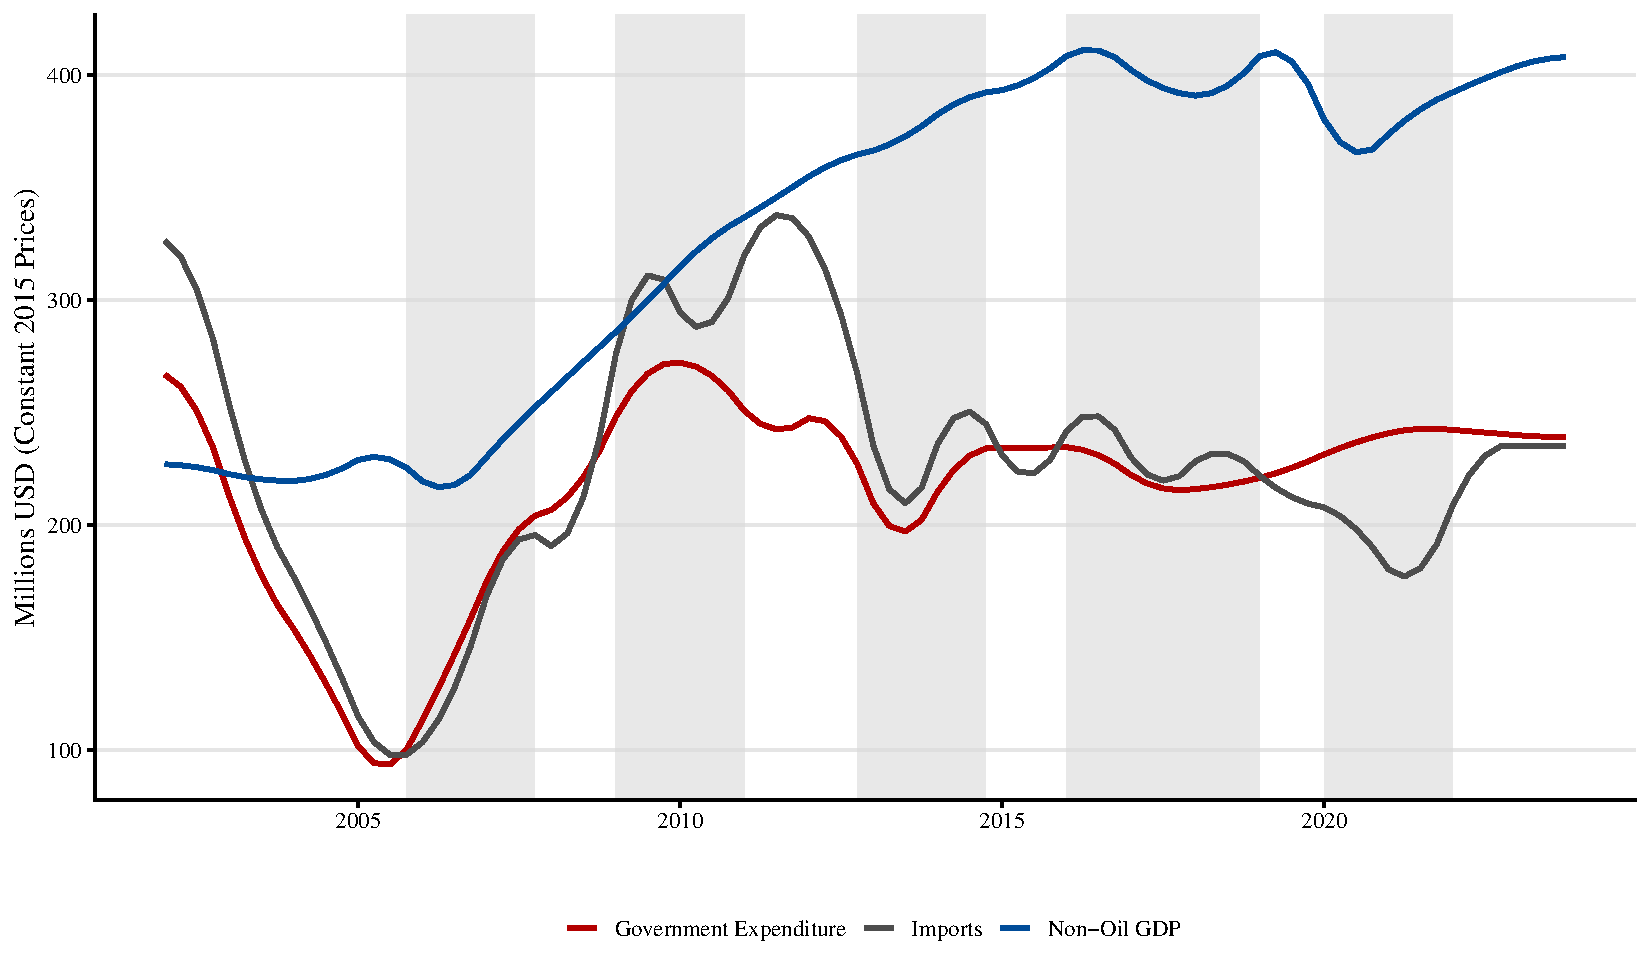
\includegraphics[width=\textwidth]{../graphics/figure_1_macro_levels.pdf}
  \caption{Niveles}
\end{subfigure}\hfill
\begin{subfigure}[t]{0.49\textwidth}
  \centering
  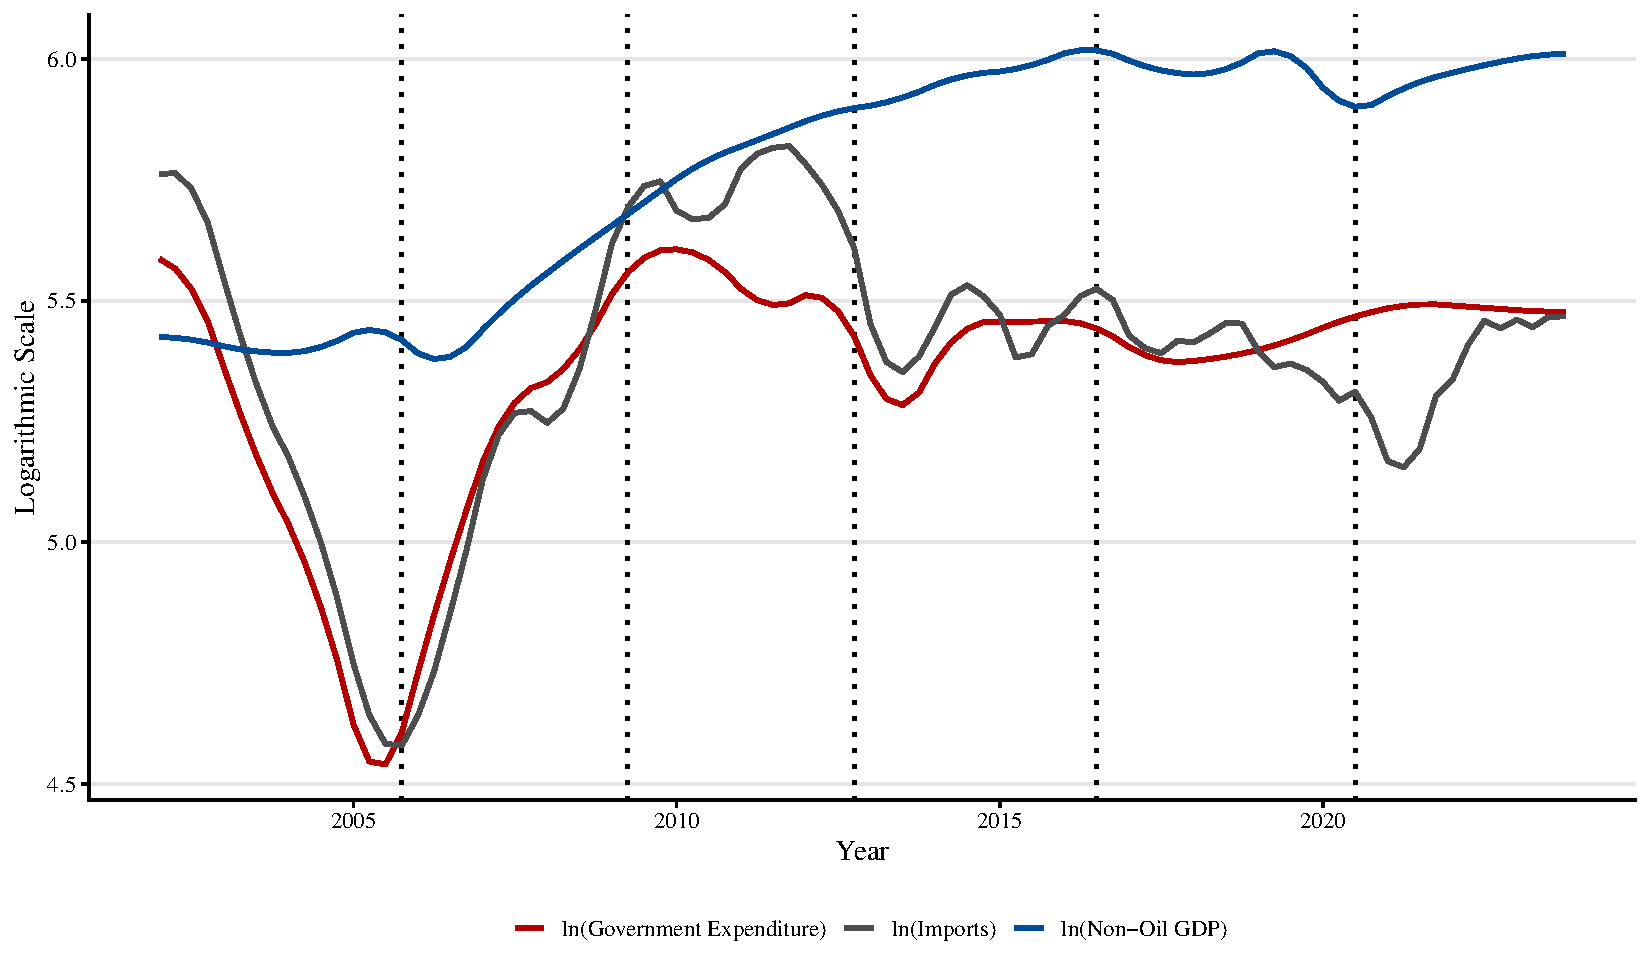
\includegraphics[width=\textwidth]{../graphics/figure_2_macro_log.pdf}
  \caption{Logaritmos y quiebres}
\end{subfigure}
\caption{Evolución de las principales series macroeconómicas de Timor-Leste, 2002Q1--2023Q4. Las áreas grises (panel izquierdo) marcan ventanas de eventos; las líneas punteadas (panel derecho) marcan quiebres seleccionados por BIC. Unidades: millones de USD a precios constantes de 2015 (gasto, PIB e importaciones). Fuente: elaboración propia con datos del ADB.}
\label{fig:macro}
\end{figure}

Los diagnósticos disponibles provienen de la corrida de
\texttt{scripts/06\_hyperparameters\_\allowbreak lag\_\allowbreak bvar\_test.R}. Esa corrida estima un
modelo de dos rezagos con la misma configuración de prior, pero su
ordenamiento interno de variables no coincide exactamente con el orden 1 ni con
el orden 2 de la especificación principal; por ello se usan como diagnósticos
de referencia y no como diagnósticos exactos de las resultados principales. La
figura~\ref{fig:estabilidad} muestra que el mayor módulo propio del
polinomio característico es 0.9929 (menor que uno), lo que sugiere un VAR
estable.

\begin{figure}[htbp]
\centering
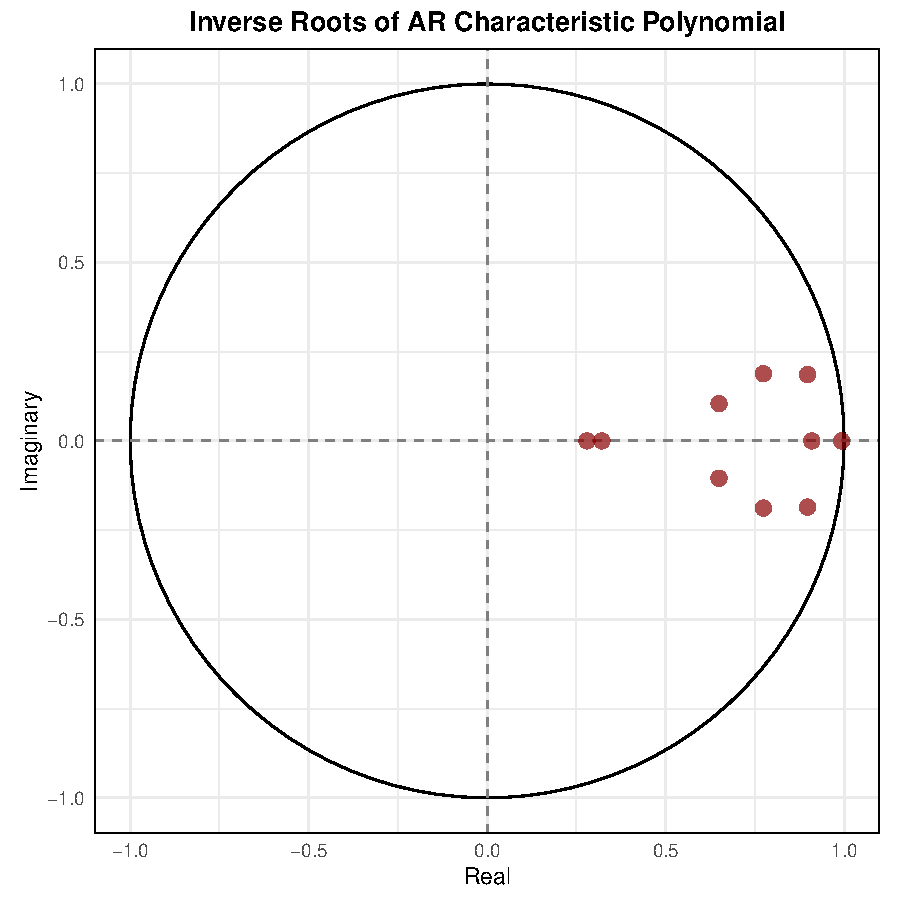
\includegraphics[width=0.55\textwidth]{../graphics/03_bvar_stability_roots.pdf}
\caption{Raíces inversas del polinomio característico del BVAR. El mayor módulo es 0.9929, inferior a uno. Fuente: elaboración propia con \texttt{scripts/06\_hyperparameters\_lag\_bvar\_test.R}.}
\label{fig:estabilidad}
\end{figure}

Con todo, los diagnósticos residuales no son plenamente satisfactorios y deben
reportarse como limitaciones. Las pruebas de Ljung--Box rechazan la ausencia de
autocorrelación en las cinco series (con $p=0.0000$ en cuatro de ellas y
$p=0.0006$ en el crédito), y las pruebas ARCH rechazan la ausencia de
heterocedasticidad en cuatro de las cinco; el IPC es la excepción, con
$p=0.235$. El propio código advierte que la
interpolación Denton--Cholette induce suavidad y autocorrelación
intrínseca, de modo que estos rechazos reflejan, al menos en parte, el
método de desagregación temporal y no solo una mala especificación del
VAR. Las pruebas de convergencia de Geweke no aprueban 5 de los 55 coeficientes
$\beta$ ni 1 de las 25 varianzas, aunque los tamaños de muestra efectivos son
cercanos a 4\,000 en las extracciones conservadas. El modelo no debe presentarse
como si todos los diagnósticos fueran satisfactorios.

\subsection{IRF puntuales al shock fiscal}
\label{sec:irf_puntual}

Los paneles de la figura~\ref{fig:irf} reportan las respuestas puntuales ante
un shock fiscal ortogonalizado de una desviación estándar del error estructural
del gasto. Para facilitar la lectura, en el texto esas respuestas se reescalan a
un aumento de 1\% del gasto y se expresan como elasticidades. Las bandas
sombreadas corresponden al intervalo posterior central del 80\% (cuantiles
0.10--0.90). Una respuesta se describe como distinta de cero solo cuando ese
intervalo excluye el cero.

\begin{figure}[htbp]
\centering
\begin{subfigure}[t]{0.49\textwidth}
  \centering
  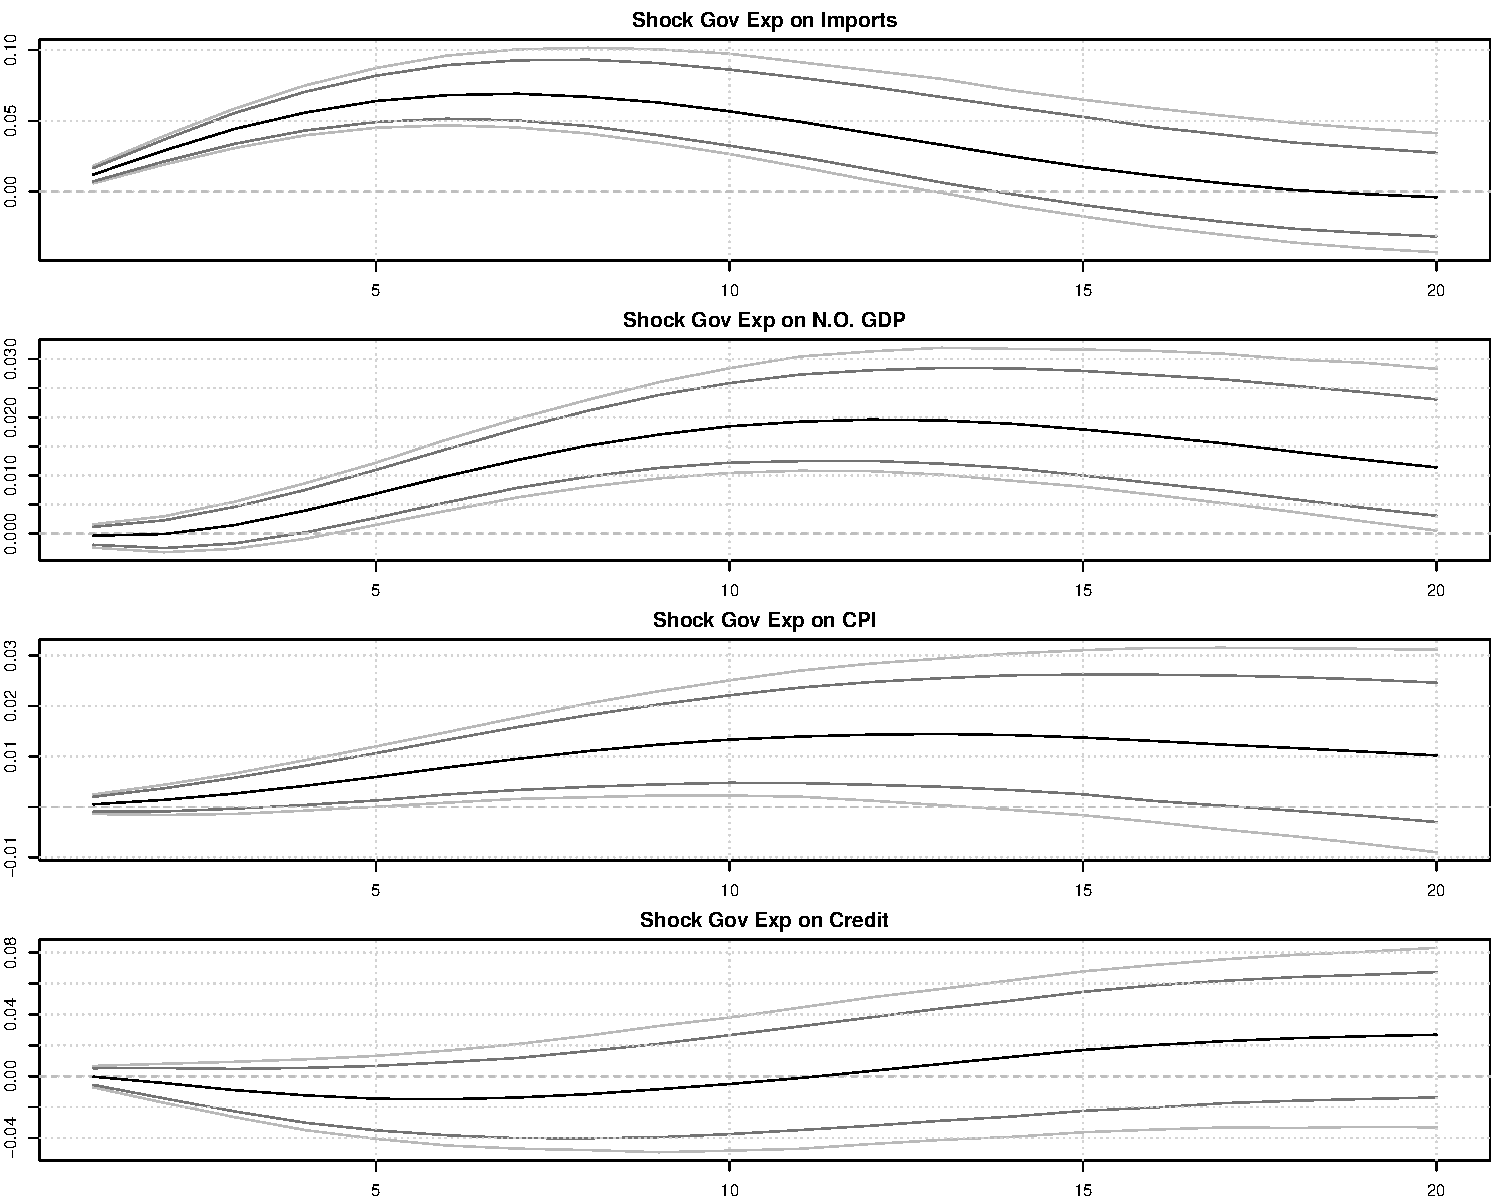
\includegraphics[width=\textwidth]{../graphics/irf_gov_shock_order_1.pdf}
  \caption{Orden 1}
\end{subfigure}\hfill
\begin{subfigure}[t]{0.49\textwidth}
  \centering
  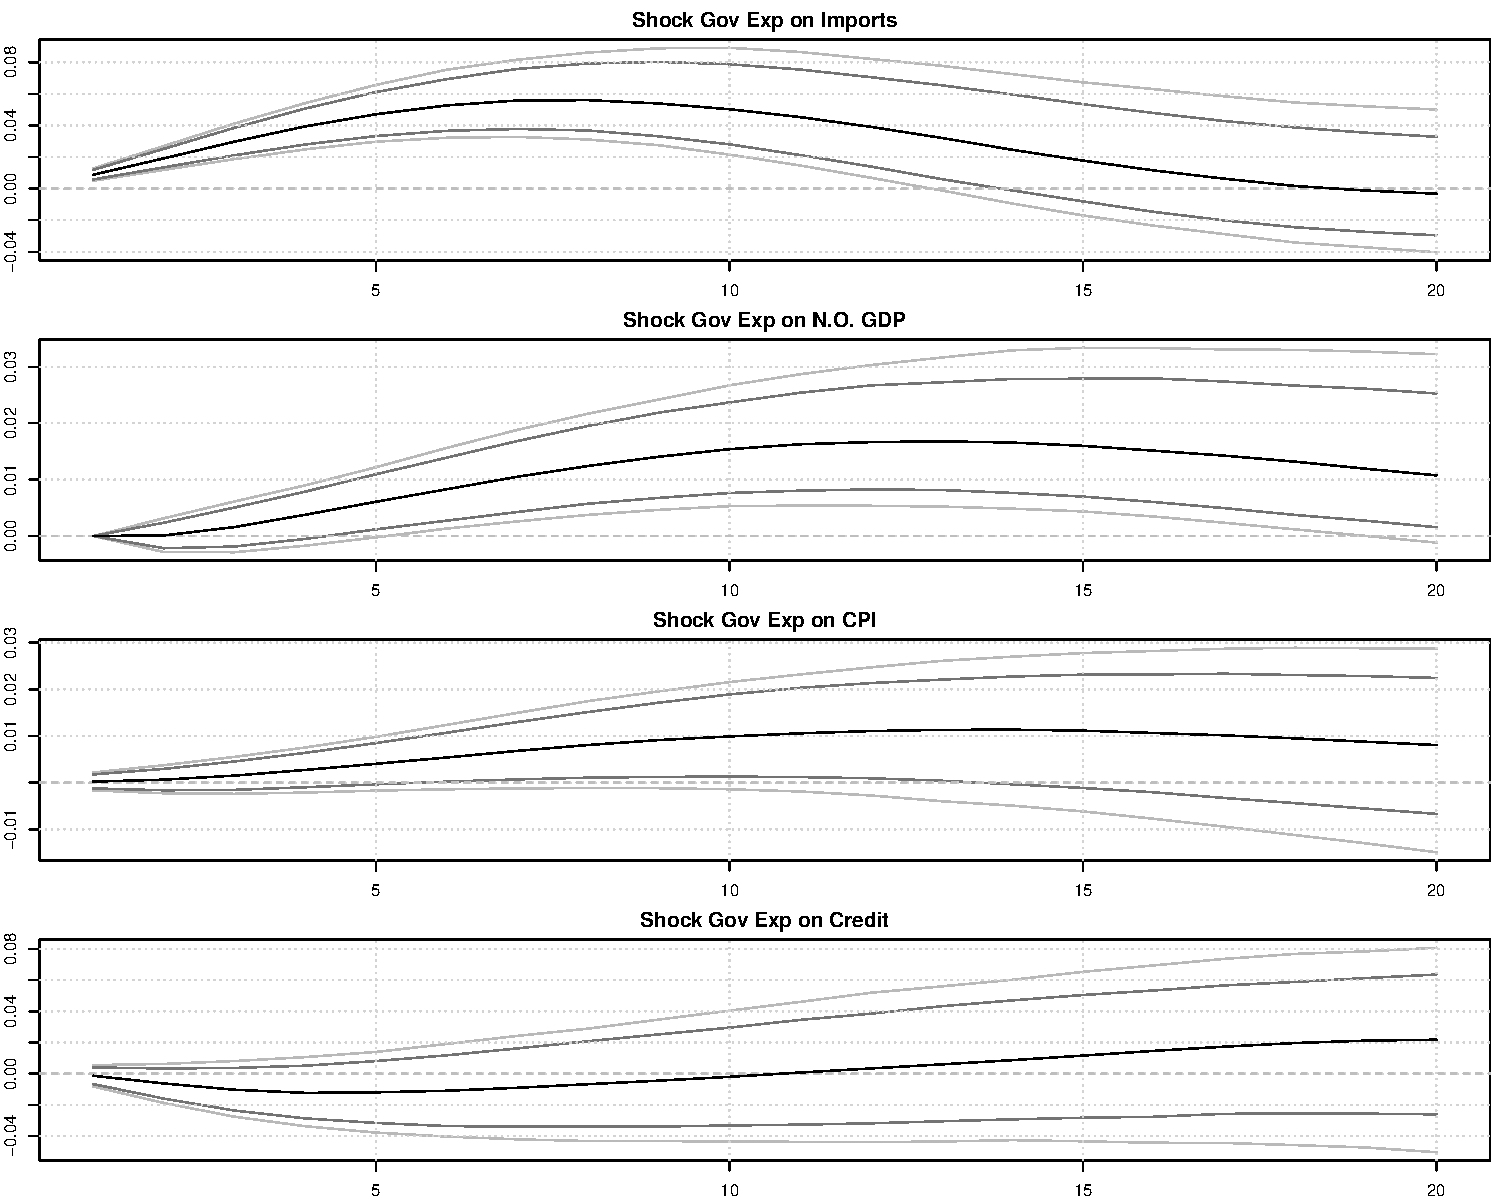
\includegraphics[width=\textwidth]{../graphics/irf_gov_shock_order_2.pdf}
  \caption{Orden 2}
\end{subfigure}
\caption{IRF puntuales ante el shock del gasto público, órdenes 1 y 2. Bandas: 68\% y 80\%. Unidades: respuesta ante un shock ortogonalizado de una desviación estándar; el texto la expresa como elasticidad ante un aumento de 1\% del gasto. Fuente: elaboración propia con \texttt{scripts/07\_irf\_fevd.R}.}
\label{fig:irf}
\end{figure}

\paragraph{Síntesis del mecanismo.}
El shock relevante es una expansión transitoria del gasto público. La respuesta
económicamente más importante es la de las importaciones: es la más rápida y de
mayor magnitud del sistema, lo que sugiere que el gasto público se ejecuta con un
alto contenido importado y que el estímulo se filtra al exterior. El PIB responde
después y de forma moderada, consistente con rezagos de absorción y
encadenamientos domésticos limitados. La respuesta de precios es pequeña e
incierta, y la del crédito no se distingue de cero, de modo que no se detecta un
canal inflacionario ni financiero. En conjunto, la evidencia es consistente con
una economía pequeña y abierta donde la absorción doméstica es limitada y la vía
externa actúa como válvula de escape del gasto público. Estas son elasticidades
condicionales a un choque estructural y a la identificación recursiva, no efectos
causales únicos.

\paragraph{Gasto público.}
La respuesta del propio gasto es positiva, persistente y relativamente precisa en
el corto y mediano plazo. En el orden 1 el intervalo del 80\% excluye el cero
entre $H{=}1$ y $H{=}12$ (y el del 68\% en la misma ventana); en el orden 2 el
intervalo del 80\% cubre $H{=}1$--$H{=}12$ y el del 68\% se extiende hasta
$H{=}13$. La mediana alcanza su máximo alrededor de $H{=}5$ (2.1\% en el orden 1 y
1.8\% en el orden 2) y se disipa hasta volver a cero hacia el final del
horizonte, cuando el intervalo contiene cero. Esto indica un shock transitorio con inercia de aproximadamente dos a tres
años, no un cambio permanente en el nivel del gasto. Económicamente, se trata de
una expansión fiscal temporal, no de un aumento permanente del tamaño del
Estado; la inercia sugiere que el impulso se ejecuta a lo largo de varios años.

\paragraph{PIB no petrolero.}
La respuesta del PIB no petrolero es positiva pero rezagada, con forma de joroba.
El intervalo del 80\% excluye el cero desde $H{=}5$ hasta $H{=}19$ en el orden 1
y desde $H{=}6$ hasta $H{=}19$ en el orden 2; el del 68\% lo hace desde $H{=}5$
hasta $H{=}20$ en ambos órdenes. La mediana máxima es una elasticidad de 0.58 en $H{=}12$ (orden 1) y 0.49 en
$H{=}13$ (orden 2): ante un aumento de 1\% del gasto, el PIB no petrolero
responde con un aumento de 0.58\% o 0.49\%. La respuesta es cualitativamente
robusta al orden, aunque su magnitud y su ventana de significancia cambian
ligeramente. Económicamente, el efecto sobre la producción doméstica es positivo
pero modesto y llega con unos tres años de rezago; esto sugiere que la capacidad
de absorción y los encadenamientos domésticos limitan el efecto de corto plazo.
Hacia $H{=}20$ la respuesta se desvanece, por lo que no se detecta un cambio
permanente en el nivel de actividad.

\paragraph{Importaciones.}
Las importaciones presentan la respuesta más rápida y de mayor magnitud del
sistema.
El intervalo del 80\% excluye el cero entre $H{=}1$ y $H{=}12$ en ambos
órdenes; el del 68\% se extiende hasta $H{=}13$ en los dos casos. La mediana máxima es una elasticidad de 2.04 en $H{=}7$ (orden 1) y 1.63 en
$H{=}8$ (orden 2): ante un aumento de 1\% del gasto, las importaciones responden
con un aumento de 2.0\% o 1.6\%. Este patrón es compatible con una alta
propensión a importar y con una fuga externa temprana del estímulo fiscal.
Económicamente, una elasticidad mayor que uno y mayor que la del PIB indica que
el gasto público tiene un alto contenido importado: el estímulo se gasta fuera
del aparato productivo doméstico antes de traducirse en producción local. En el
corto plazo, el estímulo parece ``pasar de largo'' por el aparato productivo
local.

\paragraph{IPC.}
La respuesta del IPC es positiva y pequeña, y su significancia depende del
intervalo, del horizonte y del orden. En el orden 1, el intervalo del 68\%
excluye el cero entre $H{=}5$ y $H{=}16$ y el del 80\% solo entre $H{=}7$ y
$H{=}12$. En el orden 2, el 68\% excluye cero entre $H{=}6$ y $H{=}13$, pero el
80\% no lo hace en ningún horizonte. La mediana máxima es una elasticidad de 0.41 (orden 1, $H{=}12$) y 0.33
(orden 2, $H{=}14$): 0.4\% y 0.3\%, respectivamente. Por tanto, se encuentra evidencia
moderada de una respuesta positiva de precios en el orden 1 y evidencia más
débil en el orden 2; en ambos casos la magnitud es reducida y el intervalo
del 80\% contiene cero hacia el final del horizonte. No corresponde afirmar que
``no hay inflación'', ni atribuir la respuesta a capacidad ociosa sin
evidencia directa; corresponde señalar que la respuesta estimada es
pequeña, se desvanece y es sensible al orden y al intervalo posterior
considerado. Económicamente, la respuesta pequeña y frágil sugiere que el
estímulo no genera una presión inflacionaria clara; si la demanda adicional se
satisface con importaciones en lugar de presionar una oferta local inelástica, es
esperable que no haya un brote inflacionario fuerte. La evidencia no permite
distinguir entre importaciones y capacidad ociosa.

\paragraph{Crédito privado.}
La respuesta puntual del crédito no se distingue de cero en ningún
horizonte: ni el intervalo del 68\% ni el del 80\% excluyen el cero en ninguno de
los dos órdenes. Las medianas muestran una trayectoria ligeramente negativa
en el corto plazo y ligeramente positiva al final, pero con intervalos amplios.
No hay evidencia de un desplazamiento (crowding-out) ni de un estímulo
crediticio claro. La redacción prudente es que no se encuentra evidencia
estadística de una respuesta del crédito al shock fiscal, y no que el
canal financiero esté ausente. Económicamente, no se detecta crowding-out ni
crowding-in: el financiamiento del gasto público no parece desplazar ni estimular
al sector privado local, y el canal financiero no aparece como un mecanismo
relevante de transmisión.

\subsection{IRF acumuladas}
\label{sec:irf_cum}

La figura~\ref{fig:ircum} presenta las respuestas acumuladas para los dos
órdenes. Estas magnitudes son sumas de respuestas por horizonte; se expresan
como elasticidades acumuladas y no deben leerse como cambios permanentes del
nivel.

La respuesta acumulada del gasto público es positiva y distinta de cero en
todo el horizonte, lo que refleja persistencia. La respuesta acumulada del PIB
no petrolero es positiva y distinta de cero desde $H{=}7$ (orden 1) y $H{=}8$
(orden 2). La respuesta acumulada de las importaciones es la mayor y sus
intervalos excluyen cero. En términos comparativos, la elasticidad acumulada de
las importaciones es aproximadamente 2.7 veces la del PIB en el orden 1 y 2.6
veces en el orden 2, lo que sugiere que una fracción importante del estímulo se
asocia a compras externas. Esta comparación es un cociente entre respuestas
acumuladas, no una proporción del gasto en dólares que ``se fuga''.
Económicamente, esto confirma que, acumulado en el tiempo, el canal externo
domina: por cada punto de respuesta acumulada del PIB, las importaciones
responden 2.6--2.7 puntos. El efecto doméstico es positivo pero limitado.

La respuesta acumulada del IPC es positiva con el intervalo del 80\% fuera de
cero solo en la ventana media, y la del crédito no es distinguible de cero en
ningún horizonte en ninguno de los dos órdenes.

\begin{figure}[htbp]
\centering
\begin{subfigure}[t]{0.49\textwidth}
  \centering
  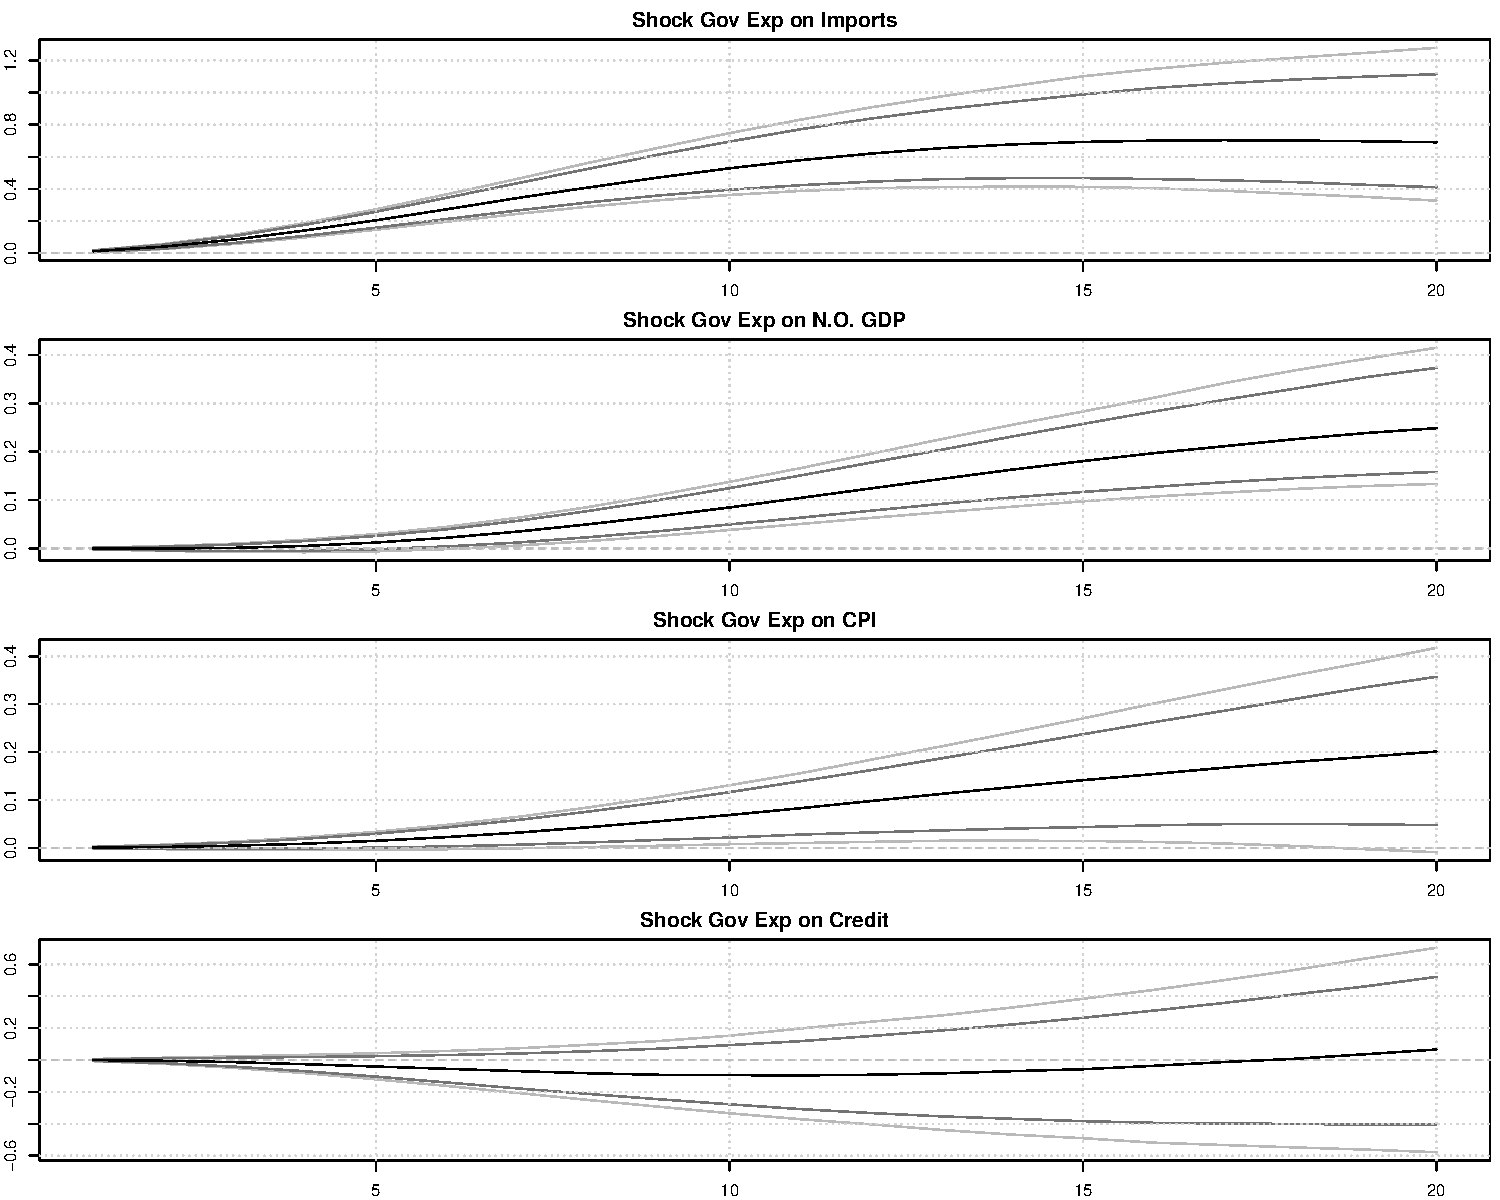
\includegraphics[width=\textwidth]{../graphics/irf_cum_gov_shock_order_1.pdf}
  \caption{Orden 1}
\end{subfigure}\hfill
\begin{subfigure}[t]{0.49\textwidth}
  \centering
  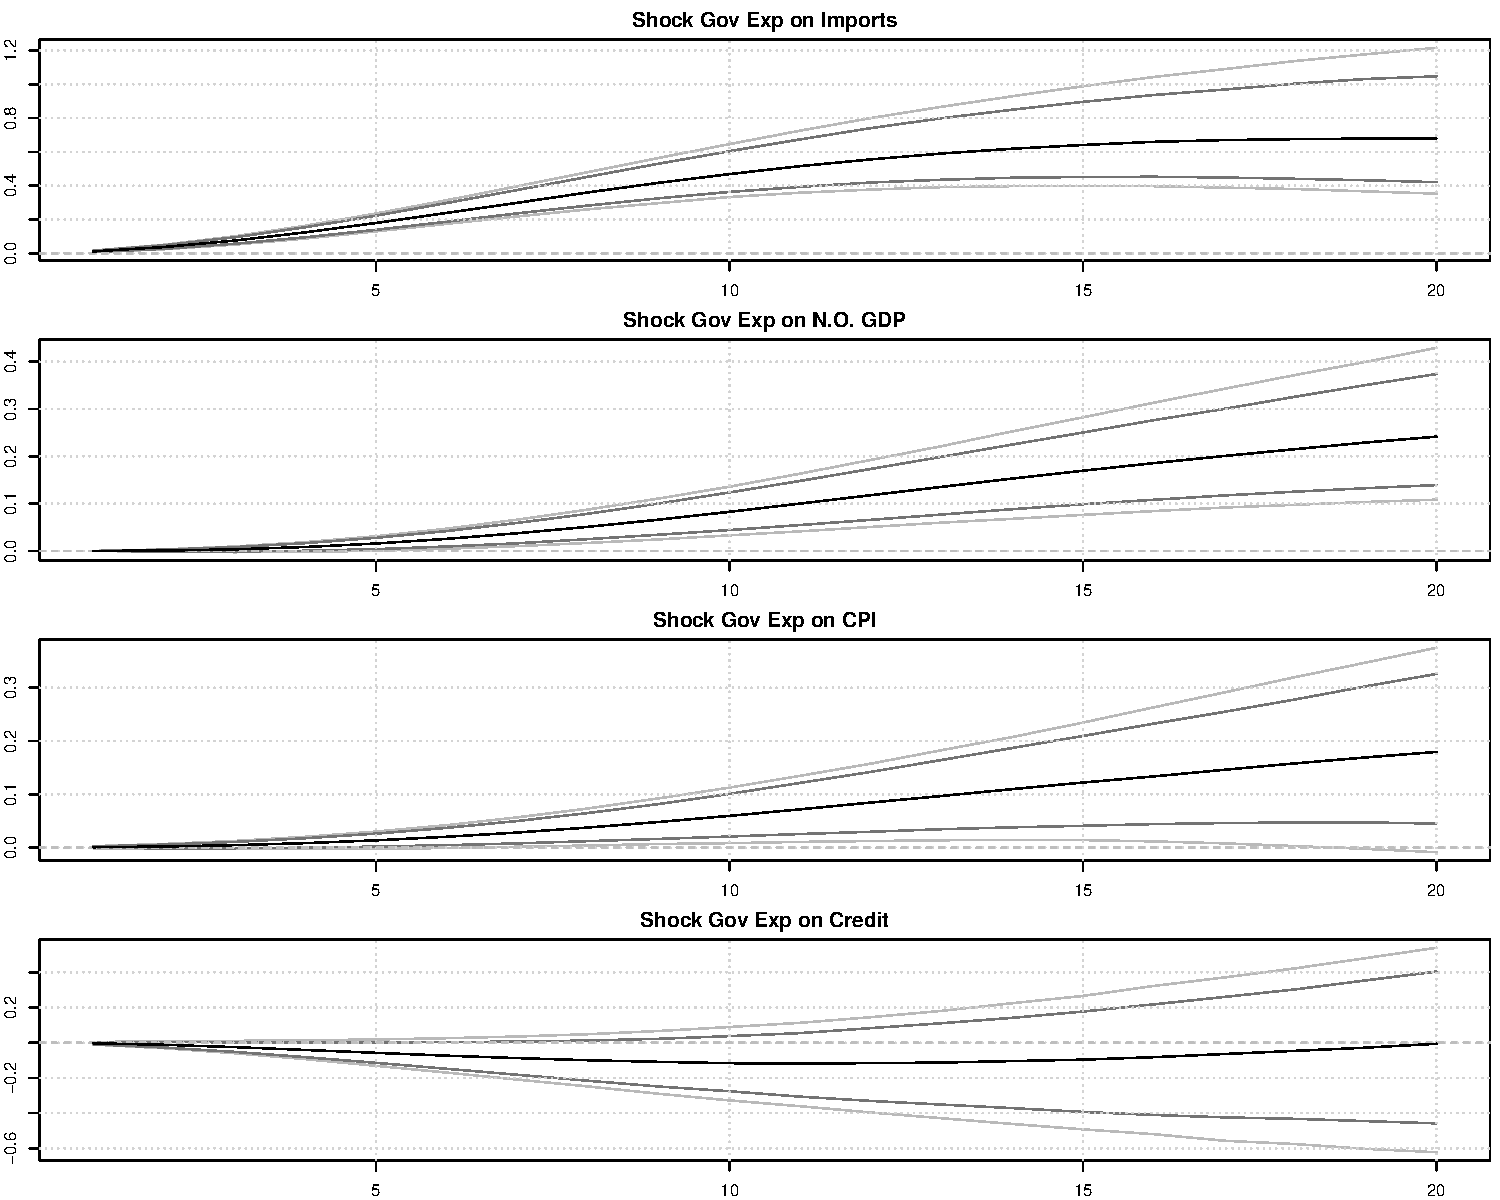
\includegraphics[width=\textwidth]{../graphics/irf_cum_gov_shock_order_2.pdf}
  \caption{Orden 2}
\end{subfigure}
\caption{IRF acumuladas ante el shock del gasto público, órdenes 1 y 2. Unidades: respuesta acumulada ante un shock ortogonalizado de una desviación estándar; el texto la expresa como elasticidad acumulada ante un aumento de 1\% del gasto. Fuente: elaboración propia con \texttt{scripts/07\_irf\_fevd.R}.}
\label{fig:ircum}
\end{figure}

\subsection{FEVD}
\label{sec:fevd}

La figura~\ref{fig:fevd} presenta la proporción de la varianza del error de
pronóstico de cada variable atribuida al shock del gasto público en
$H{=}1$, $H{=}5$, $H{=}10$ y $H{=}20$. Se reportan medianas.


\begin{figure}[htbp]
\centering
\begin{subfigure}[t]{0.49\textwidth}
  \centering
  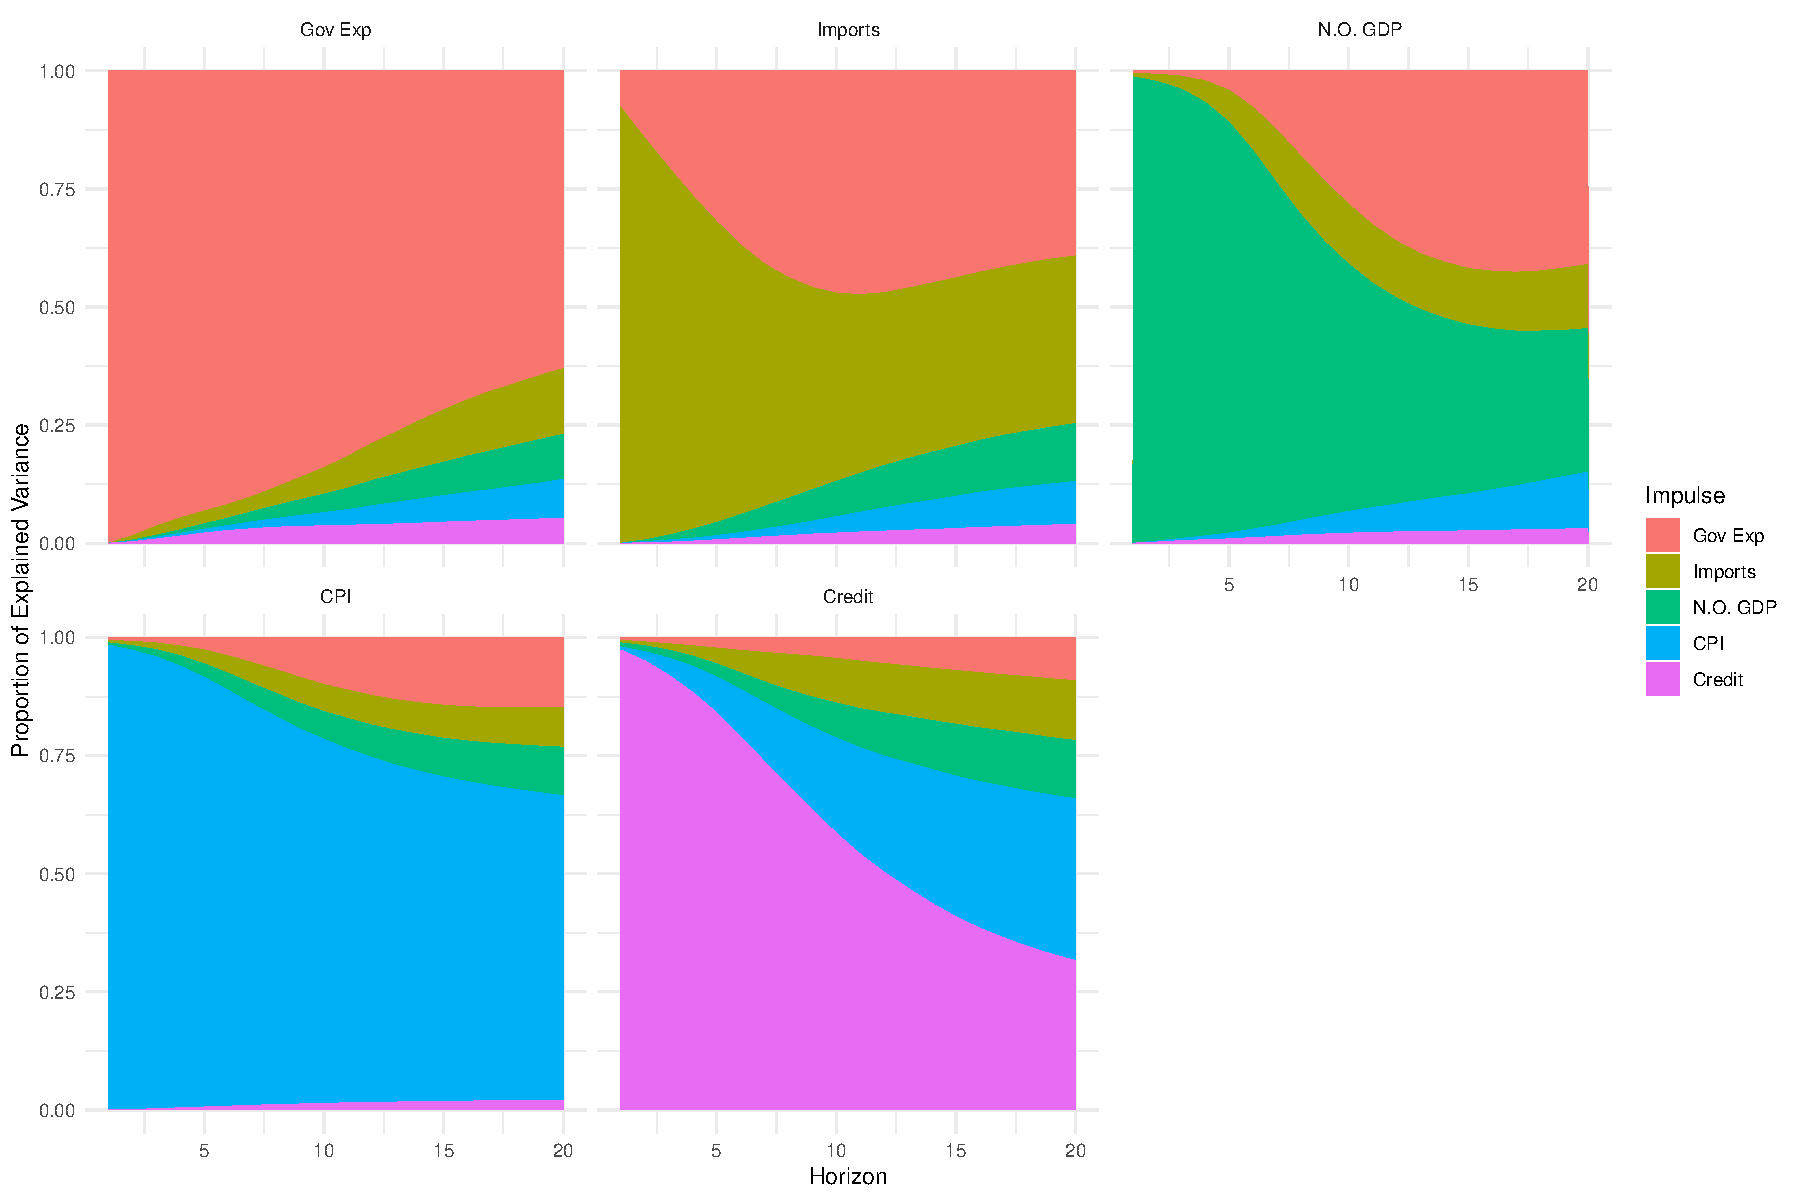
\includegraphics[width=\textwidth]{../graphics/fevd_median_order_1.pdf}
  \caption{Orden 1}
\end{subfigure}\hfill
\begin{subfigure}[t]{0.49\textwidth}
  \centering
  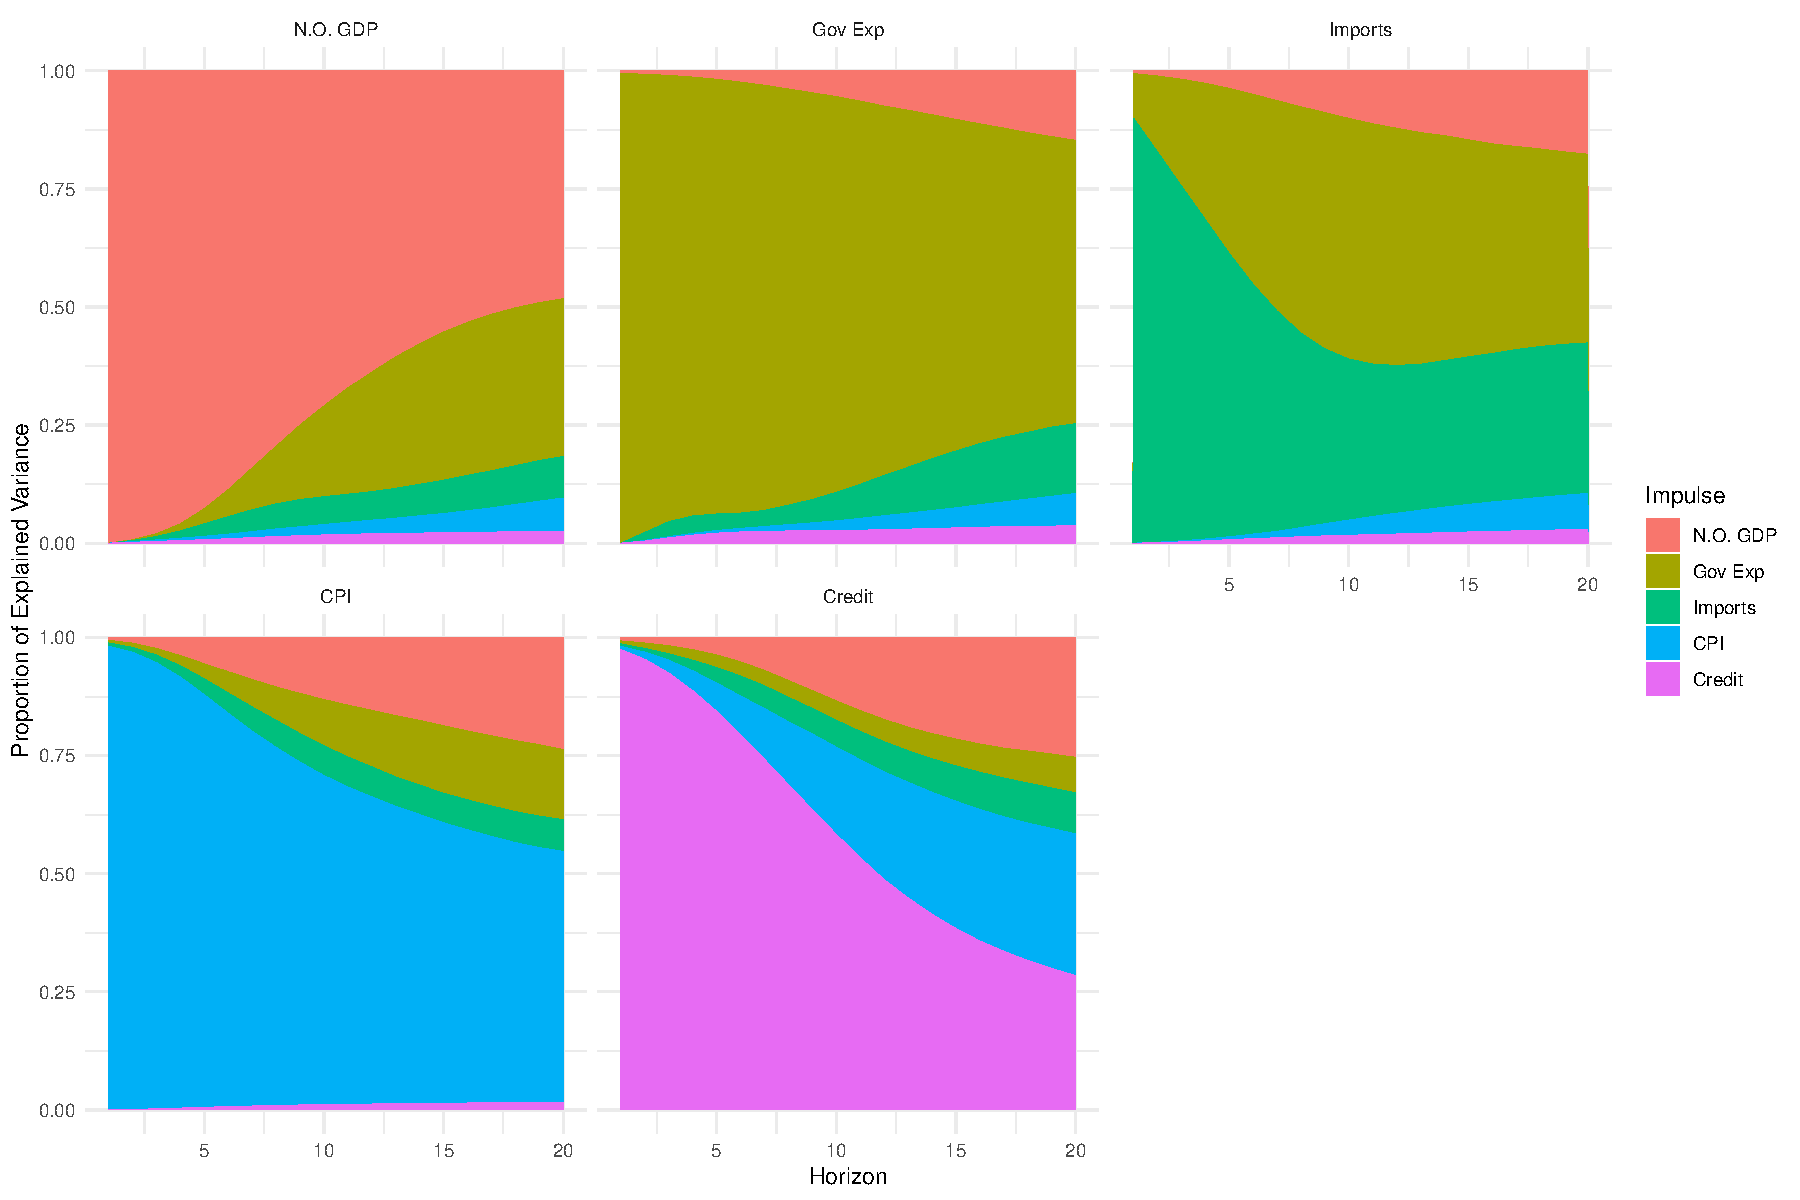
\includegraphics[width=\textwidth]{../graphics/fevd_median_order_2.pdf}
  \caption{Orden 2}
\end{subfigure}
\caption{FEVD: contribución del shock fiscal a la varianza del error de pronóstico (medianas). Fuente: elaboración propia con \texttt{scripts/07\_irf\_fevd.R}.}
\label{fig:fevd}
\end{figure}

En $H{=}1$, el shock fiscal explica casi toda la varianza del propio gasto
(99--100\%) y una fracción pequeña de la varianza de las importaciones
(8--9\%); por construcción de la identificación, explica cero (orden 2) o
casi cero (0.5\%, orden 1) de la varianza del PIB en el impacto. En $H{=}20$, el
shock fiscal explica 35.5\% de la varianza del PIB no petrolero en el orden 1 y
23.6\% en el orden 2; 34.8\% y 27.1\% de la varianza de las importaciones; 12.6\%
y 10.2\% de la del IPC; y 8.0\% y 6.9\% de la del crédito. La contribución
del propio gasto a su varianza cae a 56.5\% en el orden 1 y 50.3\% en el orden 2
en $H{=}20$, lo que indica retroalimentación parcial de otras variables. La
FEVD es cualitativamente similar entre órdenes, con diferencias moderadas en
las magnitudes. Económicamente, el shock fiscal es un determinante relevante
pero no dominante de la volatilidad del PIB y de las importaciones; su baja
contribución a la varianza del crédito confirma que el canal financiero es
marginal. La contribución comparable entre PIB e importaciones sugiere que la
volatilidad fiscal se transmite tanto por la actividad doméstica como por la
demanda externa.

\clearpage

\subsection{Comparación entre identificaciones}
\label{sec:comparacion}

Los resultados cualitativamente consistentes entre órdenes son: la
persistencia transitoria del gasto público; la respuesta positiva y distinta de
cero del PIB no petrolero a partir del quinto o sexto trimestre; la respuesta
inmediata, positiva y mayor de las importaciones; la respuesta positiva pero
pequeña del IPC en el corto y mediano plazo; y la ausencia de una respuesta del
crédito distinguible de cero. La contribución del shock fiscal a la varianza del
PIB en $H{=}20$ es 35.5\% en el orden 1 y 23.6\% en el orden 2; la de las
importaciones es 34.8\% y 27.1\%, respectivamente.

Los resultados sensibles al orden son de magnitud y de ventana de significancia,
no de signo. La ventana del PIB comienza en $H{=}5$ en el orden 1 y en $H{=}6$
en el orden 2; la del IPC se reduce hasta desaparecer al 80\% en el orden 2. La
magnitud puntual del gasto difiere porque cada corrida tiene su propia escala de
shock; por eso las comparaciones se hacen en elasticidades. El crédito no cambia
su conclusión básica entre órdenes: no hay respuesta distinguible de cero. Los
cambios en la ventana de significancia son esperables al alterar las restricciones
contemporáneas y no invalidan la dinámica general de transmisión: las
importaciones siguen reaccionando más y antes que el PIB, el PIB sigue
respondiendo con rezago y el crédito sigue sin respuesta. En ningún caso
corresponde interpretar que un orden ``prueba'' el mecanismo causal; ambos son
sensibilidades bajo supuestos recursivos.


\subsection{Reproducibilidad}
\label{sec:repro}

Todo el código, los datos procesados y los resultados están disponibles en el
repositorio público
\url{https://github.com/Emerson-nic/Timor-Leste-fiscal-bvar}. El
\texttt{README} documenta la estructura del proyecto, las fuentes, el orden de
ejecución de los scripts y la compilación del documento con LuaLaTeX y Biber.
El tablero interactivo con los resultados principales está disponible en
\url{https://connect.posit.cloud/em3r/content/01a068c1-99da-638d-1ba0-1254293e5a61}.

Invito a las personas interesadas a revisar el repositorio y a aportar mejoras,
correcciones o extensiones que contribuyan a una discusión más informada sobre
la política fiscal en Timor-Leste.

\section{Consideraciones finales}
\label{sec:final}

El BVAR trimestral sugiere que el gasto público de Timor-Leste tiene un
efecto transitorio sobre sí mismo y una asociación positiva, rezagada y
moderada con el PIB no petrolero. Las importaciones responden antes y con mayor
magnitud, lo que es compatible con un canal de fuga externa. No se encuentra
evidencia de una respuesta del crédito privado y la respuesta de precios,
aunque positiva en el corto y mediano plazo, es pequeña y sensible al
intervalo posterior. Estas conclusiones son evidencia condicionada al modelo,
al prior, a la desagregación temporal de series anuales y al orden recursivo
de identificación. No deben interpretarse como una prueba de un orden causal
único. La
principal recomendación metodológica es corregir la exportación de
FEVD para que los cuantiles se calculen sobre participaciones ya normalizadas por
extracción. La base de importaciones ya está conciliada entre archivos y
la semilla del script principal está fijada; conviene añadir una semilla
explícita antes del segundo modelo para reproducir cada orden de forma
independiente.

\printbibliography[title={Referencias}]


\appendix
\renewcommand{\thesection}{Anexo \Alph{section}}

Los anexos reúnen material complementario que no es necesario para seguir el
argumento principal, pero que documenta decisiones metodológicas y permite
auditar los resultados. El~\ref{sec:anexo_trademap} justifica la elección
del método de desagregación temporal. El~\ref{sec:anexo_irf} presenta las
matrices completas de IRF ortogonalizadas para los dos órdenes, que permiten ver
todas las respuestas del sistema y no solo las del shock fiscal.

\section{Prueba del indicador trimestral de Trade Map}
\label{sec:anexo_trademap}

El código comentado en \texttt{scripts/02\_dessagregation.R} estima una
desagregación de Chow--Lin con las importaciones trimestrales de \emph{Trade Map}
como indicador de las importaciones anuales. La desagregación temporal busca
obtener una serie trimestral consistente con el total anual. Chow--Lin usa una
serie trimestral relacionada para distribuir ese total; si el indicador aporta
información, su coeficiente debería ser distinto de cero y el ajuste debería
mejorar. La tabla~\ref{tab:anexo_trademap} reproduce la salida relevante: el
coeficiente del indicador es 0.1706 con un error estándar de 0.2959
($p=0.571$) y el $R^2$ ajustado es $-0.0328$. Es decir, el indicador no mejora
la estimación y añade ruido. Por eso se descartó y se usó la desagregación
univariada de Denton--Cholette, que preserva el total anual sin imponer una
relación de alta frecuencia que los datos no respaldan. Esta decisión importa
porque una serie trimestral mal interpolada podría contaminar las IRF y la
FEVD.

\begin{verbatim}
q_imports_model <- tempdisagg::td(imports_real ~ ts_imports_q,
                                  method = "chow-lin-maxlog",
                                  conversion = "sum")
\end{verbatim}

\begin{table}[htbp]
\centering
\small
\begin{threeparttable}
\caption{Prueba de Chow--Lin con el indicador trimestral de \emph{Trade Map}}
\label{tab:anexo_trademap}
\begin{tabular}{@{}lcccc@{}}
\toprule
Parámetro & Estimación & EE & $t$ & $p$ \\
\midrule
Intercepto & 217.7737 & 38.2836 & 5.688 & $<0.001$ \\
\texttt{ts\_imports\_q} & 0.1706 & 0.2959 & 0.576 & 0.571 \\
\bottomrule
\end{tabular}
\begin{tablenotes}\footnotesize
\item Nota: 22 observaciones anuales convertidas a 88 trimestres; conversión
de suma; método \texttt{chow-lin-maxlog}. $R^2$ ajustado: $-0.0328$;
parámetro AR(1): 0.8874. Fuente: elaboración propia con
\texttt{scripts/02\_dessagregation.R}.
\end{tablenotes}
\end{threeparttable}
\end{table}

\clearpage
\section{Matrices completas de IRF ortogonalizadas}
\label{sec:anexo_irf}

Las figuras~\ref{fig:irf_full_order_1} y~\ref{fig:irf_full_order_2} presentan
la matriz completa de funciones de impulso-respuesta para los dos órdenes.
Cada panel lleva el título ``Shock X on Y'': muestra la respuesta de la variable
$Y$ a un shock ortogonalizado de la variable $X$. A diferencia de las figuras
del texto, que se concentran en el shock fiscal, estas matrices permiten ver
todas las respuestas del sistema y comprobar si el shock de gasto público está
capturando variación de otras fuentes.

Todas las IRF del documento son ortogonalizadas: la descomposición de Cholesky
transforma los errores reducidos en shocks estructurales ortogonales. No se
reportan IRF de forma reducida. La matriz completa ayuda a distinguir el shock
fiscal de los demás: las respuestas propias muestran persistencia, mientras que
las respuestas cruzadas son, en general, más pequeñas y con intervalos más
amplios. La lectura principal sigue siendo la respuesta al shock de gasto
público; las demás celdas son un diagnóstico de consistencia y no se interpretan
como efectos causales separados.

En términos económicos, la pregunta que guía estas matrices es si el gasto de
gobierno ayuda a la economía o si se traduce principalmente en importaciones.
La respuesta es intermedia: el PIB no petrolero aumenta, pero las importaciones
aumentan antes y más, de modo que el estímulo llega a la actividad doméstica con
rezago y con una fuga externa considerable. Las respuestas dependen del orden
recursivo de Cholesky y deben leerse como evidencia condicionada, no como
causalidad estructural.

\begin{figure}[p]
\centering
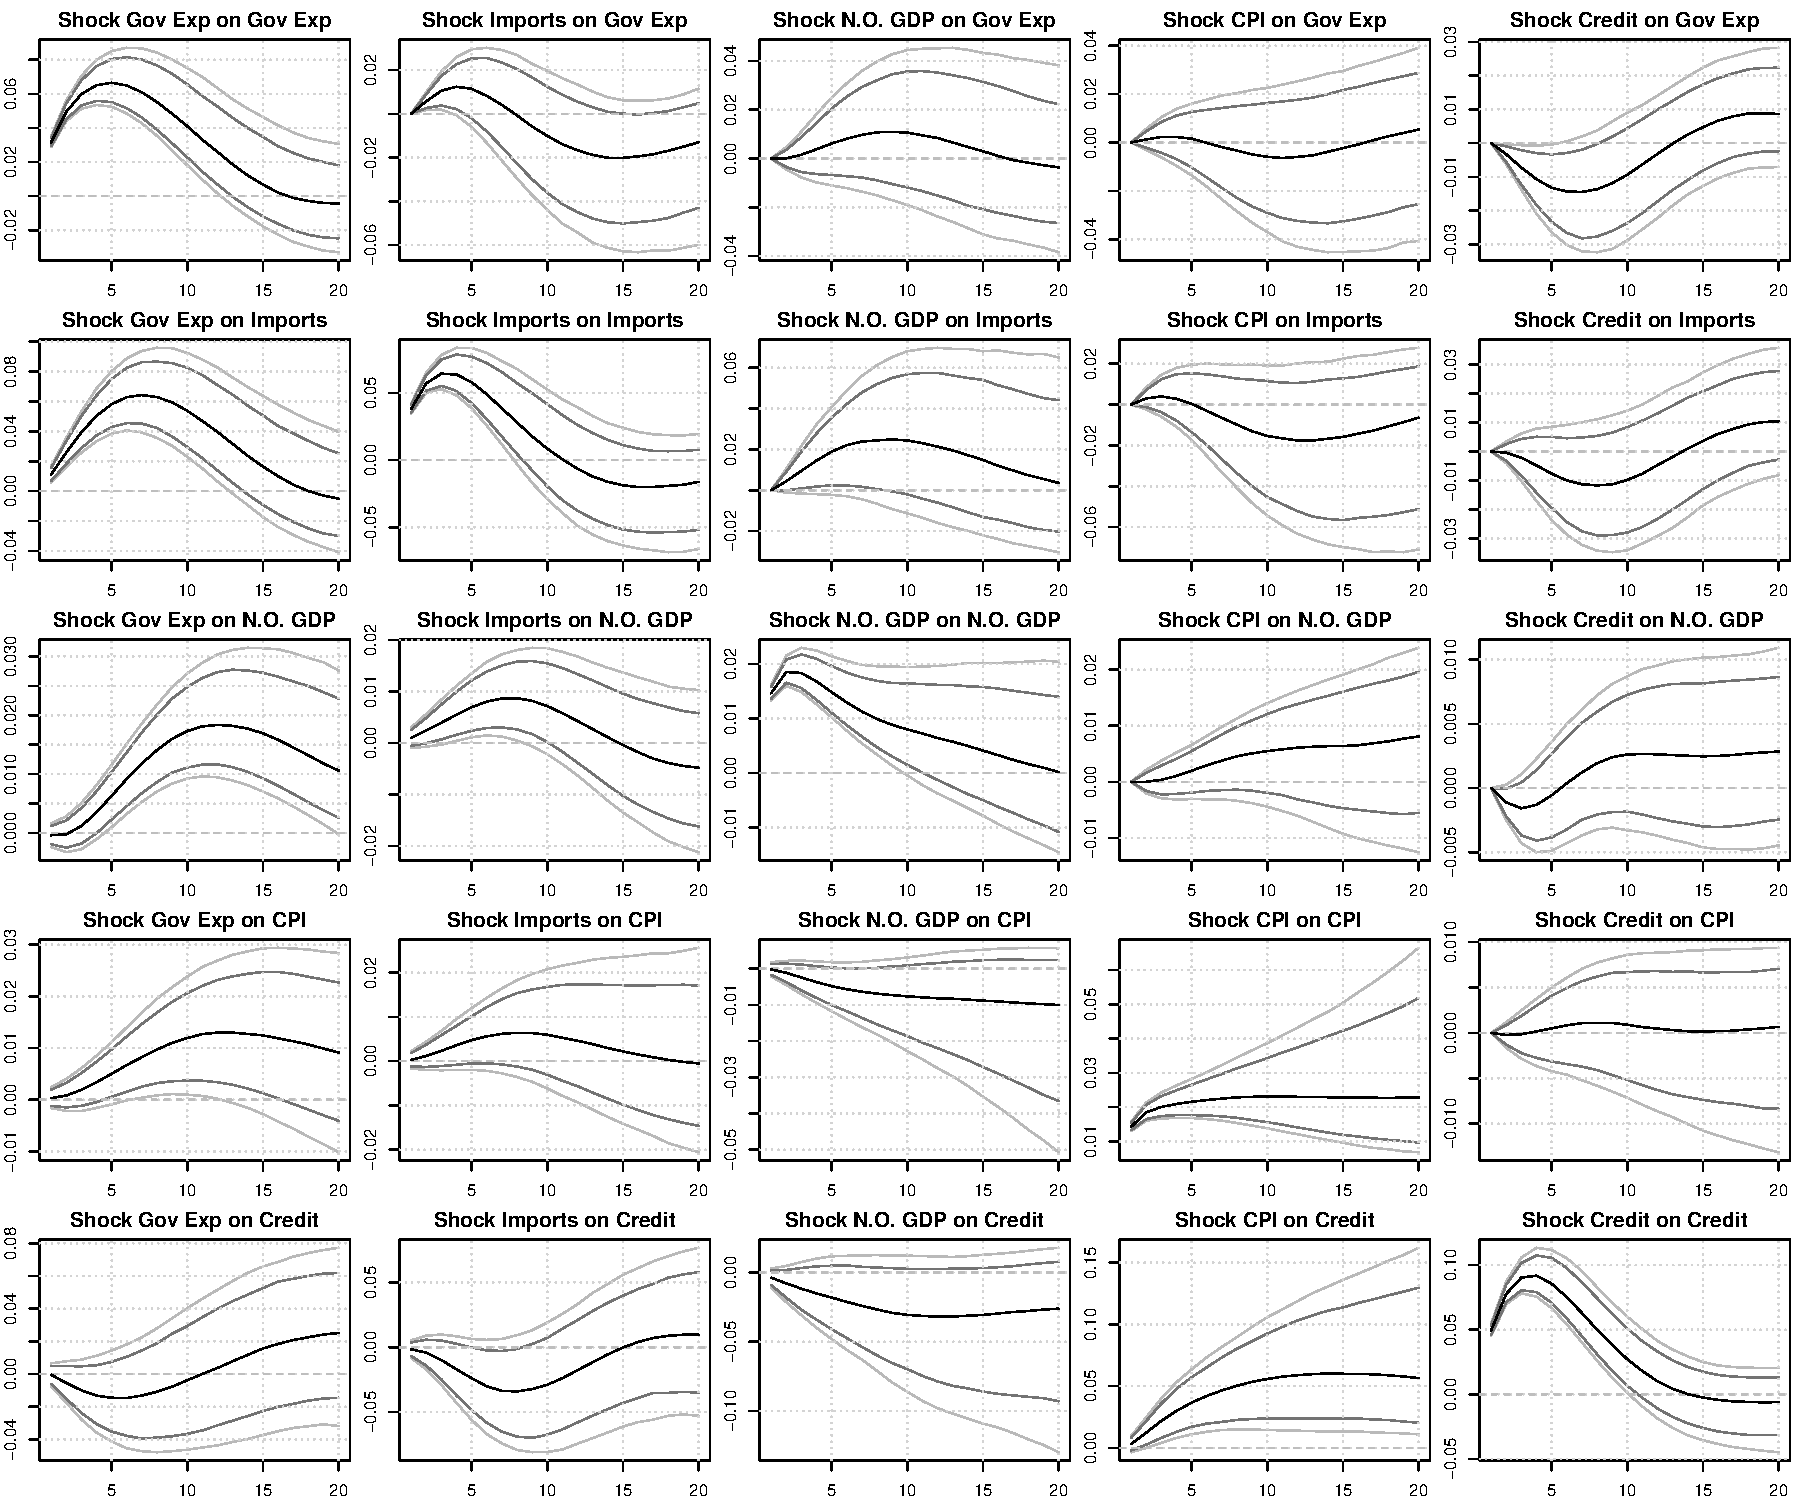
\includegraphics[width=0.95\textwidth]{../graphics/irf_full_matrix_order_1.pdf}
\caption{Matriz completa de IRF ortogonalizadas, orden 1. Cada panel muestra la
respuesta de la variable indicada después de ``on'' a un shock ortogonalizado de
la variable indicada después de ``Shock''. Bandas: 68\% y 80\%. Fuente:
elaboración propia con \texttt{scripts/07\_irf\_fevd.R}.}
\label{fig:irf_full_order_1}
\end{figure}

\begin{figure}[p]
\centering
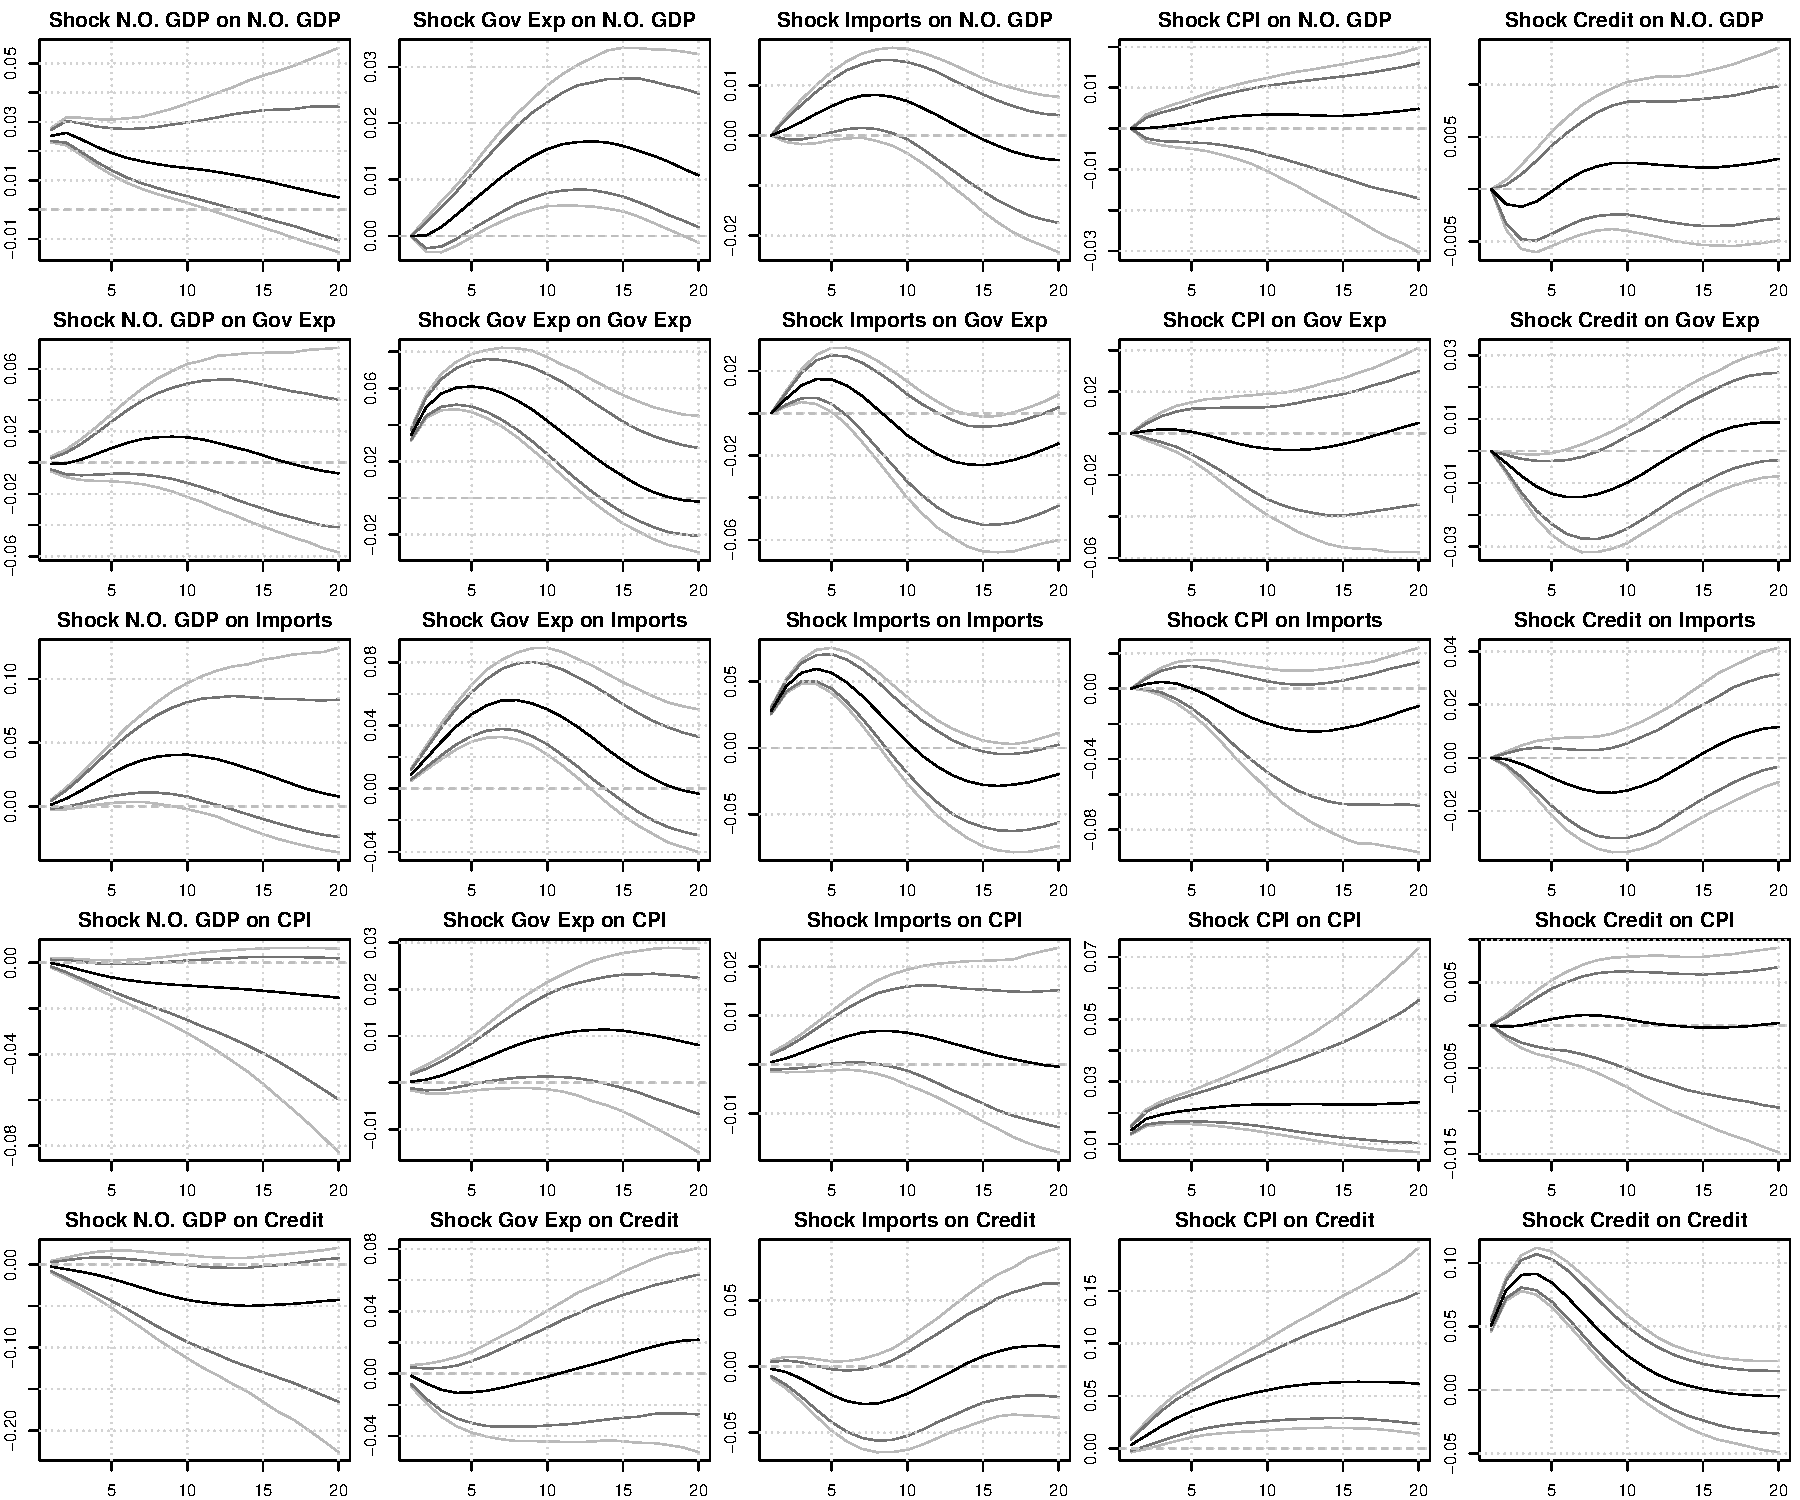
\includegraphics[width=0.95\textwidth]{../graphics/irf_full_matrix_order_2.pdf}
\caption{Matriz completa de IRF ortogonalizadas, orden 2. Cada panel muestra la
respuesta de la variable indicada después de ``on'' a un shock ortogonalizado de
la variable indicada después de ``Shock''. Bandas: 68\% y 80\%. Fuente:
elaboración propia con \texttt{scripts/07\_irf\_fevd.R}.}
\label{fig:irf_full_order_2}
\end{figure}

\end{document}
